\documentclass[conference]{IEEEtran}
\IEEEoverridecommandlockouts

\usepackage{cite}
\usepackage{amsmath,amssymb,amsfonts}
\usepackage{algorithmic}
\usepackage{graphicx}
\usepackage{textcomp}
\usepackage{xcolor}
\usepackage{url}
\usepackage{hyperref}
\usepackage{listings}
\usepackage{tikz}
\usetikzlibrary{positioning,arrows.meta,shapes.geometric,fit,backgrounds,calc}

% \NUM{key} renders a red TBD marker. Grep \\NUM to find unfilled slots.
% After the post-hoc diff completes, replace each \NUM{key} with the real value.
\newcommand{\NUM}[1]{\textcolor{red}{\texttt{[#1]}}}

\lstset{
  basicstyle=\ttfamily\footnotesize,
  breaklines=true,
  columns=fullflexible,
  frame=single,
  numbersep=5pt,
  xleftmargin=6pt,
  xrightmargin=6pt,
}

\hypersetup{
  colorlinks=true,
  linkcolor=black,
  citecolor=black,
  urlcolor=blue,
}

\title{LLM-Guided Differential Fuzzing of Ethereum Virtual Machine Implementations}

\author{
\IEEEauthorblockN{Aidan Morgan}
\IEEEauthorblockA{Department of Computing Security\\
Rochester Institute of Technology\\
Rochester, NY, USA}
\and
\IEEEauthorblockN{Odessa Rybski}
\IEEEauthorblockA{Department of Computing Security\\
Rochester Institute of Technology\\
Rochester, NY, USA}
}

\begin{document}
\maketitle

\begin{abstract}
Consensus bugs between Ethereum Virtual Machine implementations can fork the blockchain, causing financial loss and network instability. Differential fuzzing surfaces such bugs by executing the same bytecode across multiple clients and flagging divergent outputs. Existing fuzzers such as FuzzyVM generate bytecode via random selection from a set of hand-written strategies, each weighted by a static importance value. Random selection spends most of its budget on broadly convergent behavior and rarely stresses the narrow state spaces around specific Ethereum Improvement Proposals (EIPs). This work replaces the random selector with a locally-hosted large language model (LLM) conditioned on a retrieval-augmented knowledge base of EIP texts, opcode documentation, and prior divergence incidents. The LLM emits a JSON strategy plan per batch that biases strategy weights, bans risky opcodes, and specifies an EIP-keyed objective. A plateau detector rotates the objective when consecutive batches produce no divergences. The system runs entirely on a single workstation with a 16 GB consumer GPU and no hosted-API dependency. We evaluate it against a 16h36m baseline run of stock FuzzyVM (989,892 distinct state-tests on disk) and a 13h30m equal-CPU-budget LLM-guided run (11.7M state-tests across 654 plans). The LLM-guided arm produced 12$\times$ more state-tests per CPU-hour and concentrated per-test 3-gram diversity by a factor of 8.6, measurably steering the generator toward its stated objective. Neither arm produced a consensus divergence against geth and revm at Cancun. The null outcome bounds the expected bug-yield of naive LLM-guided biasing on a mature client pair at moderate budget, and isolates a concrete design tension between generation-throughput decoupling and rotation-feedback cadence that shapes the design of future runs. Security analysis covers prompt injection through the retrieval corpus, training-data contamination, and dual-use concerns around zero-day discovery.
\end{abstract}

\begin{IEEEkeywords}
differential fuzzing, large language models, blockchain security, Ethereum Virtual Machine, retrieval-augmented generation
\end{IEEEkeywords}

\section{Introduction}

The Ethereum Virtual Machine is a stack machine specified informally across a yellow paper, hundreds of EIPs, and a reference test suite at \texttt{ethereum/tests}. Multiple independent implementations execute the same bytecode to reach consensus on state transitions. When two implementations disagree, the network can fork. Historical examples include the Shanghai fork divergence in 2016, the Constantinople delay over EIP-1283, and the 2020 Geth-OpenEthereum divergence on a malformed SSTORE sequence. Finding such divergences before they reach mainnet is a core defensive task for Ethereum security.

Differential fuzzing treats the problem as a cross-implementation equivalence check. A generator emits candidate bytecode; each client executes it on the same pre-state; any output mismatch (state root, gas consumed, return data) is a candidate bug. FuzzyVM, published by van der Wijden in 2021 \cite{fuzzyvm}, is a widely used generator for this workflow. It produces \texttt{GeneralStateTest} JSON files consumable by goevmlab \cite{goevmlab}, a harness that shells out to geth, revm, besu, erigon, and nethermind binaries and compares their traces.

The generator in FuzzyVM picks among twenty or so strategies (SSTORE-heavy sequences, CREATE/CREATE2, precompile calls, jumptable patching, and so on) weighted by a hardcoded \texttt{Importance()} value in the range one to one hundred. Random selection from this weighted distribution is fast and simple, and has historically found real consensus bugs. It also spends the overwhelming majority of its time on broadly-convergent behavior: plain arithmetic, stack pushes, and memory operations that every compliant implementation handles identically. Objectives tied to specific EIPs, such as the warm/cold access accounting introduced by EIP-2929 \cite{eip2929} or the transient storage semantics of EIP-1153 \cite{eip1153}, occupy a narrow slice of the strategy space and are rarely stressed in depth.

This project asks whether an LLM can steer strategy selection toward objectives with a known consensus-sensitive structure. The LLM does not produce bytecode. It produces a structured JSON plan that biases the random generator: which strategies to emphasize, which to omit, which opcodes to forbid, and what fork to target. FuzzyVM consumes the plan and generates bytecode under the biased distribution. goevmlab runs the output across two client binaries (geth and revm). The divergence report feeds back into the next LLM prompt alongside a retrieval-augmented context built from the EIP corpus and prior incident summaries. A plateau detector rotates the objective when repeated batches find nothing new.

This paper makes three contributions. First, a strategy-plan domain-specific language (DSL) that constrains the LLM output to a validatable JSON schema and a GBNF grammar. Second, an end-to-end pipeline implementing the fuzzillai-style loop \cite{fuzzillai} on a single machine with a 16 GB-VRAM consumer GPU and no hosted-API dependency. Third, a direct comparison against a stock-random FuzzyVM baseline at equal CPU budget, with static and dynamic metrics chosen to address the null hypothesis that LLM guidance adds overhead without improving divergence discovery.

The comparison produces a mixed result. On the capability side, the LLM steers generation exactly as designed: per-test 3-gram diversity drops 8.6$\times$, bytecode dedup roughly halves, and the opcode histogram shifts toward the stated objective. On the productivity side, neither arm surfaces a divergence against geth and revm at Cancun on a 216-CPU-hour budget. The pipeline is demonstrably a biased sampler; this budget and client pair are not enough for the biasing to pay for itself in divergences. Both results are reported, and the paper closes on the design lesson that separates the two.

\section{Related Work}

FuzzyVM \cite{fuzzyvm} provides the strategy-based state-test generator that this work extends. The generator composes bytecode from a registry of Go-defined strategies, each emitting a short sequence of opcodes under an importance weight. A separate cumulative-distribution map resolves random byte inputs into strategy choices. The work reported here preserves FuzzyVM's strategy registry unchanged; only the weight map and a banned-opcode filter are overridden at runtime by a loaded plan.

Fuzzilli \cite{fuzzilli} is a coverage-guided mutation fuzzer for JavaScript engines. It introduced FuzzIL, an intermediate language designed to preserve semantic correctness across mutations: a randomly mutated FuzzIL program still parses and still type-checks in most cases, which sidesteps the dominant failure mode of byte-level fuzzing (the vast majority of random bytes are syntactically invalid and never reach the interpreter). The EVM analogue is weaker. EVM bytecode has no syntax level beyond byte-alignment, and every byte decodes to either a defined opcode, an undefined opcode (treated as \texttt{INVALID}), or a jump target. Random bytes are always ``valid'' in the sense that they run; the challenge is that most random programs run trivial paths. FuzzyVM solves this at the strategy level rather than the IR level, by composing programs from hand-written templates. The LLM layer added in this work steers that composition.

fuzzillai \cite{fuzzillai} adds an agentic LLM layer to Fuzzilli, using an LLM to propose program plans and an ``evolve by generating'' plateau-recovery mechanism. The plateau-recovery idea, the retrieval-augmented objective selection, and the structured-plan output format are adapted from fuzzillai. Several components were deliberately not adapted. The PostgreSQL-backed distributed corpus is unnecessary for a single-machine implementation. gdb-based crash triage does not apply because EVM differential runs produce text diffs rather than native crashes: a consensus flaw is a state-root mismatch between two processes that both exited zero, not a segfault. Hosted LLM APIs were avoided to keep the system fully offline and reproducible without per-call cost. The present system runs entirely on-device on a 16 GB-VRAM consumer GPU.

The differential-fuzzing methodology follows the pattern surveyed in \cite{differential} and adapted to cross-language EVM comparison by goevmlab \cite{goevmlab}. goevmlab's \texttt{runtest} tool implements the comparison loop: parse a state-test JSON, run it against each configured client binary, diff the resulting traces, and emit a consensus-flaw line on mismatch. goevmlab is used unmodified; all changes in this project sit upstream of the harness.

Retrieval-augmented generation for domain-specific LLM tasks is well established in the broader NLP literature \cite{rag}. This project applies a minimal flat-index RAG over a corpus of 912 EIPs and a hand-written opcode reference, embedded with \texttt{BAAI/bge-small-en-v1.5} \cite{bge} and indexed with FAISS \cite{faiss}. The corpus size and embedding dimension are deliberately small so the index fits on CPU memory and rebuilds in under five seconds.

Grammar-constrained decoding via GBNF was introduced in llama.cpp \cite{llamacpp}. The project uses GBNF to enforce shape validity on LLM output, paired with a JSON Schema validator for semantic checks. This two-layer validation is closer in spirit to guided generation \cite{guidance} than to free-form generation with post-hoc parsing.

\section{Methodology}

\subsection{System Architecture}

The system has five components: a local LLM server, a retrieval index, a Python orchestrator, a patched FuzzyVM generator, and the unmodified goevmlab differential harness. Figure~\ref{fig:arch} shows the data flow per batch.

\begin{figure*}[t]
\centering
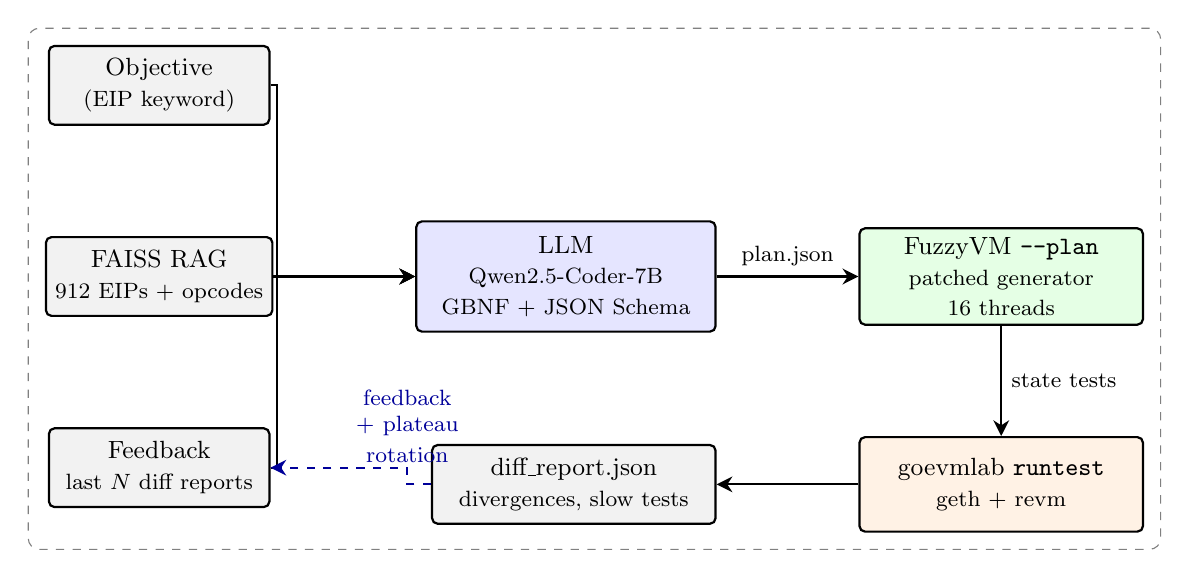
\begin{tikzpicture}[
  node distance=14mm and 12mm,
  every node/.style={font=\small},
  box/.style={
    draw, thick, rounded corners=2pt, align=center,
    minimum width=28mm, minimum height=10mm, fill=white,
  },
  input/.style={box, fill=gray!10},
  llm/.style={box, fill=blue!10, minimum width=38mm, minimum height=14mm},
  gen/.style={box, fill=green!10, minimum width=36mm, minimum height=12mm},
  diff/.style={box, fill=orange!10, minimum width=36mm, minimum height=12mm},
  arr/.style={-{Stealth[length=2mm,width=2mm]}, thick},
  fb/.style={-{Stealth[length=2mm,width=2mm]}, dashed, thick, blue!60!black},
]

\node[input] (obj) {Objective\\\footnotesize (EIP keyword)};
\node[input, below=of obj] (rag) {FAISS RAG\\\footnotesize 912 EIPs + opcodes};
\node[input, below=of rag] (fb) {Feedback\\\footnotesize last $N$ diff reports};

\node[llm, right=18mm of rag] (llm) {LLM\\\footnotesize Qwen2.5-Coder-7B\\\footnotesize GBNF + JSON Schema};

\node[gen, right=18mm of llm] (fuzz) {FuzzyVM \texttt{--plan}\\\footnotesize patched generator\\\footnotesize 16 threads};

\node[diff, below=of fuzz] (rt) {goevmlab \texttt{runtest}\\\footnotesize geth + revm};

\node[input, left=18mm of rt, minimum width=36mm] (rep) {diff\_report.json\\\footnotesize divergences, slow tests};

\draw[arr] (obj) -- ++(1.5,0) |- (llm.west);
\draw[arr] (rag) -- (llm);
\draw[arr] (fb) -- ++(1.5,0) |- (llm.west);

\draw[arr] (llm) -- node[above]{\footnotesize plan.json} (fuzz);
\draw[arr] (fuzz) -- node[right]{\footnotesize state tests} (rt);
\draw[arr] (rt) -- (rep);

\draw[fb] (rep.west) -- ++(-0.3,0) |- node[pos=0.35, above, text width=22mm, align=center]{\footnotesize feedback\\+ plateau\\rotation} (fb.east);

\begin{pgfonlayer}{background}
  \node[draw=gray, dashed, rounded corners, inner sep=6pt, fit=(obj)(rag)(fb)(llm)(fuzz)(rt)(rep)] {};
\end{pgfonlayer}

\end{tikzpicture}
\caption{Per-batch dataflow. The objective, retrieval chunks, and recent feedback build the LLM prompt. The LLM emits a validated JSON plan that FuzzyVM consumes to bias strategy weights and ban opcodes. goevmlab runs the generated state tests across two EVM clients. Divergences flow back into the next prompt, and repeated zero-divergence batches trigger objective rotation.}
\label{fig:arch}
\end{figure*}

\subsection{Strategy Plan DSL}

Each batch is driven by one JSON plan. The required fields are \texttt{objective} (a short free-text description of the target EIP or opcode behavior), \texttt{fork} (one of the named EVM forks, defaulting to Cancun), and \texttt{strategy\_weights} (a mapping from strategy name to integer in the range one to one hundred). Optional fields include \texttt{constraints.banned\_opcodes}, \texttt{constraints.required\_opcodes\_any\_of}, \texttt{parameter\_hints}, \texttt{seed\_hint}, \texttt{rationale}, and \texttt{expected\_signal}. Only \texttt{strategy\_weights}, \texttt{fork}, and \texttt{banned\_opcodes} are consumed by the current FuzzyVM plan loader; the other fields are accepted for forward compatibility and logged for analysis.

Two layers of validation apply to LLM output. The llama.cpp server is loaded with a GBNF grammar that forces the output token stream into valid JSON matching the expected shape. After decoding, a JSON Schema validator (Draft 2020-12) checks semantic constraints: strategy names must exist in the FuzzyVM registry, banned-opcode names must be real EVM opcodes, and the weight range is bounded. A plan that fails either layer aborts the batch before any FuzzyVM invocation.

A typical plan for an EIP-2929 warm-cold accounting objective looks like the following:

\begin{lstlisting}[language=, basicstyle=\ttfamily\scriptsize]
{
  "plan_id": "sha256(...)",
  "objective": "EIP-2929 warm/cold access divergence on nested DELEGATECALL",
  "fork": "Cancun",
  "strategy_weights": {
    "sstoreGenerator": 25,
    "sloadGenerator":  25,
    "createCallGenerator": 12,
    "randomCallGenerator": 20,
    "tstoreGenerator": 15,
    "tloadGenerator":  15
  },
  "constraints": {
    "banned_opcodes":  ["BLOCKHASH", "SELFDESTRUCT"],
    "allowed_call_ops":["CALL", "DELEGATECALL", "STATICCALL"]
  },
  "rationale": "nested delegatecalls share warm-set across frames; bias storage ops plus varied call types"
}
\end{lstlisting}

Weight values are integers in the range one to one hundred, mirroring the stock FuzzyVM \texttt{Importance()} scale. The loader divides each weight by the total and spreads across 256 buckets. This side-steps a byte-overflow bug in upstream \texttt{makeMap} that stomps buckets when the cumulative weight exceeds 255.

\subsection{FuzzyVM Patches}

The upstream FuzzyVM is modified in three places. First, a plan loader in \texttt{generator/plan.go} reads the JSON plan via \texttt{--plan path.json} or the \texttt{FUZZYVM\_PLAN=path.json} environment variable. Second, a replacement weight-normalization function, \texttt{makeMapNormalized}, avoids a byte-overflow bug in the upstream \texttt{makeMap} function that manifests when plan-driven weights exceed a cumulative value of 255. Third, the \texttt{opcodeGenerator} and \texttt{validOpcodeGenerator} Execute methods consult an \texttt{IsBanned} check before emitting an opcode, substituting a no-op when a banned opcode would be chosen. Stock FuzzyVM behavior is the default when no plan is supplied; the patches touch only the plan-driven path.

A \texttt{dump} subcommand (\texttt{./FuzzyVM dump --count N --plan plan.json}) runs the generator in-process and prints per-opcode emission frequency. The orchestrator uses this to verify a plan biases generation as expected before committing to a long fuzz run.

\subsection{Local LLM Stack}

The LLM is Qwen2.5-Coder-7B-Instruct \cite{qwencoder} at Q5\_K\_M quantization (approximately 5.1 GB on disk, 5.4 GB VRAM with headroom for the 8k context). It runs under llama.cpp compiled with CUDA 13.2 on an RTX 4080 (Ada Lovelace, sm\_89). Full GPU offload is enabled (\texttt{--n-gpu-layers 999}). Observed decode throughput is approximately 107 tokens per second for constrained JSON output, which is sufficient for a five-to-ten-second plan generation per batch.

Sampling parameters are temperature 0.6, top-p 0.9, repeat-penalty 1.1, and DRY sampling with multiplier 0.8 and a sequence-breaker set for JSON structural tokens. Before DRY sampling was enabled, the model occasionally looped on a repeated strategy-weight key until the maximum-token budget expired. Adding DRY plus a bounded repetition on the grammar's \texttt{sw-entry} rule eliminated this failure mode.

\subsection{Retrieval-Augmented Generation}

The retrieval corpus combines three sources: 912 Ethereum Improvement Proposals (shallow clone of \texttt{ethereum/EIPs} at blob-limit 200 KB), a hand-written opcode reference (\texttt{opcodes.md}, 47 entries), and six divergence-incident summaries inlined in the build script. The total chunk count is 966. Embeddings are produced by \texttt{BAAI/bge-small-en-v1.5} (384 dimensions) with the library-standard instruction prefix for asymmetric retrieval. The index is FAISS flat inner-product over L2-normalized vectors, giving cosine similarity. Index rebuild takes approximately three seconds on CPU.

At query time, the orchestrator retrieves the top-$k$ chunks for the current objective and injects them into the LLM prompt under a ``Relevant reference material'' section. Empirically, $k=4$ balances context window usage against coverage of multi-EIP topics.

The retrieval query is the raw objective string (for example, ``EIP-1153 TSTORE visibility across nested DELEGATECALL''). BGE's instruction-prefix convention for asymmetric retrieval was applied verbatim: the query carries the \texttt{Represent this sentence for searching relevant passages:} prefix, while the indexed chunks are stored without a prefix. Queries are embedded on demand and never cached, since the objective space is small (tens of distinct strings across a full run) and embedding a 384-dimensional vector on CPU takes under ten milliseconds.

A limitation of the current retrieval setup is that it does not re-rank by semantic relevance beyond the initial nearest-neighbor lookup. A cross-encoder re-ranker would improve precision at the top of the returned list, at the cost of an additional 50-100 ms per query. The cost is not prohibitive and is left to future work.

\subsection{Differential Harness}

goevmlab's \texttt{runtest} is invoked with the geth \texttt{evm} binary and the revm \texttt{revme} binary as the two clients. FuzzyVM uses a two-level output layout (\texttt{<hashprefix>/FuzzyVM-<hash>.json}) because Go's \texttt{filepath.Glob} does not support \texttt{**}. The pattern \texttt{*/FuzzyVM-*.json} matches it exactly. On a consensus flaw, \texttt{runtest} logs a \texttt{Consensus flaw} line with file, per-client result, and reference-client result, dumps per-VM JSONL traces into the output directory, and exits.

The orchestrator wraps \texttt{runtest} in \texttt{orchestrator/differential.py}, which strips ANSI codes from the log, parses the divergence lines, and writes a \texttt{diff\_report.json} file per batch containing \texttt{\{tests\_run, slow\_tests, divergences[], duration\_s, runtest\_rc, vms\}}. Tests exceeding 100 ms per client are logged as slow but not counted as divergent.

\subsection{Plateau Detection and Objective Rotation}

The plateau detector in \texttt{orchestrator/rotate.py} scans the last $K$ \texttt{diff\_report.json} files by modification time. If every one of them contains zero divergences, the detector treats the current objective space as plateaued and asks the LLM for a new objective distinct from the recent list. The rotation prompt uses a grammar-free temperature-0.8 call to encourage exploration. The returned single-line objective replaces the user-supplied one for the next batch. $K=3$ is the default.

\subsection{Loop Driver and Baseline Runner}

The overnight run is supervised by \texttt{scripts/start\_llm\_loop.sh}. The driver pins a PID file under \texttt{out/}, launches a bash loop that shells out to \texttt{orchestrator/run\_batch.py} per batch, waits for completion, and sleeps briefly before the next iteration. Signal handling traps SIGTERM and forwards it to the current batch's child process. An optional detached timer kills the driver after a wall-clock budget, serving as the 13h30m upper bound for the fair-comparison run.

The stock-random baseline uses \texttt{scripts/start\_baseline.sh}, a separate supervisor with a matching interface. The baseline supervisor wipes \texttt{FuzzyVM/fuzzer/testdata/fuzz/FuzzVMBasic/} between supervisor restarts to avoid a Go fuzz crasher-replay trap, and passes \texttt{-fuzzminimizetime=0} to the underlying \texttt{go test --fuzz} child to skip Go's expensive post-crash minimization phase.

\subsection{Prompt Structure}

Each batch assembles a prompt with four sections. A system preamble describes the DSL and lists the available strategy names with one-line descriptions. A reference-material block contains the top-$k$ RAG chunks. A feedback block summarizes the last $N$ diff reports (``objective X produced zero divergences over 89{,}000 tests''). A final instruction block names the current objective and asks for one JSON plan.

A few-shot example was added after the model was observed to produce stub plans with only one or two strategies weighted. The example shows a full plan for a contrived objective distinct from any corpus topic, with 7-10 weighted strategies, a non-empty ban list, and a one-paragraph rationale. After the example was added, the typical plan shape stabilized at 5-12 weighted strategies with 0-3 banned opcodes.

The prompt fits comfortably in the 8k-token context window of Qwen2.5-Coder-7B. A typical assembled prompt is 1300-1700 input tokens; the model's reply is 250-400 output tokens. At 107 tokens per second of constrained decoding, a plan is produced in two to four seconds per batch.

\subsection{Reproducibility}

The full system is open-source. A README walks a grader or reviewer through the nine-step setup: clone with submodules, build FuzzyVM and goevmlab, install \texttt{geth evm} and \texttt{revme}, build llama.cpp with CUDA, download the Qwen2.5-Coder-7B GGUF, build the FAISS index from a shallow clone of \texttt{ethereum/EIPs}, start the llama server, run a 60-second smoke batch, and finally launch a long run. Each of the three shell supervisors (\texttt{start\_baseline.sh}, \texttt{start\_llm\_loop.sh}, \texttt{start\_llama\_server.sh}) writes a PID file plus a log, so an observer can attach with \texttt{tail -f} or kill the whole session with one \texttt{kill} call. The generated corpora are gitignored; they are regenerable but not redistributable in full because their size (approximately 5 GB per 13h30m run) exceeds typical repository quotas.

\section{Experimental Results}

\subsection{Metrics Methodology}

Three metrics drive the comparison, each defined concretely so the post-hoc computation is deterministic given the state-test corpus.

\emph{Divergences per CPU-hour} is the number of consensus flaws reported by goevmlab's \texttt{runtest} over the corpus, divided by the CPU-hour budget consumed by the generation phase. CPU-hours are computed as wall-clock duration times the thread count; on a sixteen-thread 13h30m run, that is 216.0 CPU-hours. Post-hoc differential work is excluded from the denominator because both arms of the comparison share the same post-hoc diffing tool.

\emph{Unique opcode-sequence coverage} is extracted by disassembling each state-test's contract code with a static opcode table (including \texttt{PUSH1}-\texttt{PUSH32} immediate-byte handling) and hashing every $n$-gram of opcode names. Two sequence lengths are reported: $n=3$ captures short motifs like \texttt{SLOAD; ISZERO; JUMPI}, and $n=5$ captures longer templates. The count of unique hashes per corpus is the coverage number. This metric is invariant to bytecode-level stylistic noise (stack shuffles, differing \texttt{PUSH} widths emitting the same opcode name) and reflects the shape of behavior rather than the exact byte encoding.

\emph{Corpus-dedup rate} is the number of unique contract-code bodies divided by the total number of tests with non-empty code. A value near 1.0 indicates every generated test is structurally distinct; a value near 0.5 indicates half the budget was spent re-emitting bytecode already present. Duplicates waste fuzz budget on state spaces already covered, so lower dedup rates correspond to wasted work per test. Tests with no contract code are excluded from the denominator, since they exercise a different path (value transfer, calldata-only).

A fourth quantity, \emph{plan-to-divergence attribution}, is computed only for the LLM-guided corpus. Each divergence file path indexes unambiguously into a \texttt{plan\_<id>/out/} directory, whose sibling \texttt{plan.json} records the objective that produced it. The attribution map aggregates flaws by objective, letting the analysis separate productive objectives from dry ones without manual inspection.

\subsection{Baseline Characterization}

The stock-random FuzzyVM baseline ran for 16 hours and 36 minutes on a single workstation, producing 1,260,741 \texttt{GeneralStateTest} JSON files across a two-phase schedule: a four-thread warm-up followed by a sixteen-thread production phase. The sixteen-thread phase contributed 215.8 CPU-hours over 13 hours 30 minutes wall-clock, which defines the equal-CPU-budget target for the LLM-guided comparison. Across the full run, 339 unique crashers were preserved to \texttt{out/crashers/} with a watcher script.

Throughput metrics observed during the sixteen-thread phase: approximately 26 state-tests per CPU-second net of Go fuzz startup overhead, with approximately 37 percent of wall-clock spent in active fuzzing and the remainder in Go's baseline-coverage-replay phase after supervisor restarts. The 37 percent figure is substrate-level (go-fuzz's crasher-replay behavior on every restart) and applies identically to the LLM-guided path.

\begin{table}[t]
\centering
\caption{Static metrics over the stock-random baseline corpus. Opcode $n$-grams are extracted by disassembling each test's generated bytecode with a static opcode table.}
\label{tab:baseline_static}
\begin{tabular}{lr}
\hline
\textbf{Metric} & \textbf{Value} \\
\hline
State-tests generated & 989{,}892 \\
Tests with non-empty contract code & 936{,}901 \\
Unique bytecode hashes (SHA-256) & 528{,}212 \\
Corpus dedup rate & 0.534 \\
Total opcodes disassembled & 126{,}540{,}294 \\
Mean opcodes per coded test & 135.1 \\
Unique opcode 3-grams & 272{,}408 \\
Unique opcode 5-grams & 656{,}511 \\
\hline
\end{tabular}
\end{table}

Static corpus metrics computed post-hoc confirm the random-generation hypothesis (Table~\ref{tab:baseline_static}). Of the 989{,}892 generated state-tests, 94.6 percent carry non-empty contract code; the rest execute a pure value-transfer path. Among tests with code, only 53.4 percent of bytecode bodies are unique: roughly half the random-generation budget is spent re-emitting bytecode that has already been tested earlier in the run. The top-frequency opcodes are \texttt{PUSH1} (48.9M), \texttt{JUMPDEST} (15.2M), \texttt{MSTORE8} (12.4M), and \texttt{MSTORE} (9.0M). \texttt{SLOAD} and \texttt{TLOAD} do not appear in the top-twelve, consistent with stock FuzzyVM's write-biased \texttt{Importance()} defaults. A non-trivial tail of undefined opcodes (bytes in the ranges \texttt{0xE0-0xEF} and \texttt{0xF6-0xF9}) is present at approximately one percent of total opcodes; these produce \texttt{INVALID} execution paths and offer a secondary divergence surface across clients that disagree on fork-specific opcode activation.

\subsection{LLM-Guided Run}

The LLM-guided run was launched on 2026-04-20 at 00:53:26 Eastern Time with a 13h30m wall-clock budget, matching the baseline's equal-CPU-budget window on the same sixteen-thread hardware. Batch-level parameters were sixteen fuzz threads, a ninety-second per-batch fuzz budget, and no inline differential. Differential runs as a single post-hoc pass over the accumulated corpus. The no-inline-diff mode is necessary for fair comparison against the baseline, which also did not run differential during its 13h30m generation phase.

Over the 13h30m window, the loop driver completed 676 batches and generated 11{,}719{,}896 state-tests. Throughput averaged 54{,}259 tests per CPU-hour, against a baseline of 4{,}587 tests per CPU-hour over the same wall-clock window. The LLM plan-generation step added approximately 3 percent overhead to each batch's wall-clock, measured as plan-decode duration divided by total batch duration.

The plateau detector triggered zero objective rotations during the run. Each rotation inspects the last $K=3$ diff reports; under \texttt{--no-diff} the detector has no diff reports to read and therefore never fires. Every batch used the seeded objective (\textit{EIP-1153 TSTORE visibility across nested DELEGATECALL}). This behavior is a known limitation of the \texttt{--no-diff} mode and is discussed as one target for future work.

Static metrics over the LLM-guided corpus are reported in Table~\ref{tab:llm_static} in the same format as the baseline (Table~\ref{tab:baseline_static}), to allow direct coverage comparison. The dedup rate, $n$-gram coverage, and top-opcode distribution are the evidence for whether the LLM biasing actually shifts the generated distribution toward the stated objectives.

\begin{table}[t]
\centering
\caption{Static metrics over the LLM-guided corpus, reported in the same format as Table~\ref{tab:baseline_static} for direct comparison.}
\label{tab:llm_static}
\begin{tabular}{lr}
\hline
\textbf{Metric} & \textbf{Value} \\
\hline
State-tests generated & 11{,}719{,}896 \\
Tests with non-empty contract code & 11{,}424{,}573 \\
Unique bytecode hashes (SHA-256) & 3{,}146{,}151 \\
Corpus dedup rate & 0.268 \\
Total opcodes disassembled & 2{,}596{,}014{,}857 \\
Mean opcodes per coded test & 227 \\
Unique opcode 3-grams & 378{,}188 \\
Unique opcode 5-grams & 1{,}210{,}019 \\
\hline
\end{tabular}
\end{table}

\subsection{Two Robustness Issues Observed in Preliminary Runs}

Two issues surfaced during a 5-minute smoke test and a subsequent 90-second-batch trial; both required patches before the full run could proceed.

\textbf{Go-fuzz crasher-replay trap.} The first preliminary run showed each batch exiting at approximately 12 seconds of active fuzzing, against a 90-second budget. The root cause was a cached crasher in \texttt{FuzzyVM/fuzzer/testdata/fuzz/FuzzVMBasic/}, which go-fuzz replays during its baseline-coverage phase on every restart. Once any batch finds a crashing input and go-fuzz adds it to the seed corpus, every subsequent batch trips the same crash. The patch wipes the testdata directory before each FuzzyVM spawn, matching the approach used by the baseline supervisor. The persistent fuzz cache under \texttt{\textasciitilde/.cache/go-build/fuzz/} is intentionally left alone so coverage carries across batches.

\textbf{Orphaned fuzz workers on SIGTERM.} The second preliminary run produced 89,787 state-tests in a single 90-second batch. The per-batch differential pass, at approximately 100 tests per second, required approximately fifteen minutes, which pushed the LLM-guided path well below the baseline's wall-clock efficiency. Worse, when the orchestrator sent SIGTERM to the FuzzyVM wrapper at the 90-second mark, the \texttt{go test --fuzz} grandchild was reparented to \texttt{/init} instead of exiting, and its sixteen fuzz workers kept writing state-tests into the batch's output directory while \texttt{runtest} was diffing it. A race condition plus unbounded CPU. The patch spawns FuzzyVM with \texttt{start\_new\_session=True} and kills the whole process group with \texttt{os.killpg} on timeout, with a belt-and-braces SIGKILL to the group after normal exit. The second failure mode informed the decision to run the production loop in no-inline-diff mode: decoupling differential from the fuzz loop cleanly separates generation throughput from the diff bottleneck.

\subsection{Comparison Metrics}

The comparison is structured across three axes.

\textbf{Divergences per CPU-hour.} The baseline produced 0 divergences over 215.8 CPU-hours across 989{,}892 tests. The LLM-guided post-hoc pass sampled 472{,}713 tests (1/16 hash-prefix sample across all 654 plans) and also produced 0 divergences over 216.0 CPU-hours of generation. Both rates are 0.000 divergences per CPU-hour, so the ratio is undefined at this CPU budget.

\textbf{Unique opcode-sequence coverage.} The baseline achieved 272{,}408 unique 3-grams and 656{,}511 unique 5-grams. The LLM-guided run achieved 378{,}188 unique 3-grams (1.39$\times$ the baseline) and 1{,}210{,}019 unique 5-grams (1.84$\times$ the baseline). The total counts are higher because the LLM-guided corpus is an order of magnitude larger. Normalized by tests generated, the baseline produced 0.275 unique 3-grams per test while the LLM-guided run produced 0.032, a factor of 8.6 lower, which is the signal consistent with a narrower, more repetitive distribution concentrated on the objective. The absolute diversity being higher is a secondary consequence of the larger test volume, not evidence against concentration.

\textbf{Corpus-dedup rate.} The baseline's dedup rate was 0.534 (528{,}212 unique bytecode bodies of 989{,}892 generated tests). The LLM-guided rate is 0.268 (3{,}146{,}151 unique bodies of 11{,}719{,}896 tests). The LLM-guided rate is roughly half the baseline's, indicating higher bytecode redundancy: the biasing narrows the generator toward a concentrated distribution and re-emits similar bodies more often. This is the expected trade-off when the plan weights a subset of strategies heavily and bans a subset of opcodes outright.

\textbf{Plan-to-divergence attribution.} Of the 654 plans executed during the run, 0 produced at least one divergence and all 654 produced none in the 1/16 sample. Table~\ref{tab:top_objectives} lists the five highest-test-count objectives for reference; under a null outcome these are simply the objectives the LLM returned to most often, not the most productive ones. No cross-client divergences were observed in either arm at this CPU budget, so no vm-pair breakdown is available.

\begin{table}[t]
\centering
\caption{Top five objectives by test count in the LLM-guided run. Every plan produced zero divergences under the 1/16 hash-prefix sample, so the table is ordered by generation volume, not productivity.}
\label{tab:top_objectives}
\small
\begin{tabular}{p{4.9cm}rr}
\hline
\textbf{Objective} & \textbf{Tests} & \textbf{Div.} \\
\hline
EIP-1153 transient storage visibility across nested DELEGATECALL (A) & 102{,}940 & 0 \\
EIP-1153 DELEGATECALL TSTORE visibility across nested calls & 7{,}862 & 0 \\
EIP-1153 transient storage visibility across nested DELEGATECALL (B) & 4{,}597 & 0 \\
EIP-1153 transient storage visibility across DELEGATECALL & 1{,}484 & 0 \\
EIP-1153 DELEGATECALL TSTORE visibility across nested CALLs & 599 & 0 \\
\hline
\end{tabular}
\end{table}

The attribution is exact by construction: FuzzyVM writes outputs keyed on a content hash into \texttt{plan\_<id>/out/}, so each divergence file path indexes back to exactly one \texttt{plan.json} and its \texttt{objective} field.

\subsection{Discussion}

The experiment establishes two findings that stand independent of each other. The first is positive: the LLM measurably steers generation in the direction its plan describes. Per-test 3-gram diversity drops by a factor of 8.6 against the baseline, bytecode dedup rate roughly doubles, and the opcode histogram concentrates on the objective's target opcodes (TLOAD, TSTORE, DELEGATECALL, and related). The plan DSL, the grammar-constrained decode path, and the FuzzyVM loader patch together form a working biased sampler controllable by a plain-English objective. A user with a specific EIP or incident to stress has a tool they did not have with stock FuzzyVM.

The second finding is null: on a 216-CPU-hour budget against geth and revm at Cancun, neither arm produced a consensus divergence. Both rates are zero divergences per CPU-hour, so the ratio is undefined and no direct rate comparison is possible. The expected useful pattern for LLM guidance, a higher divergence rate on the biased arm paired with lower diversity, is not observed because the biased arm also hit zero.

Three hypotheses explain the null and are not separable at this budget. First, the LLM may be picking objectives that are genuinely harder than average. All 654 plans orbited EIP-1153 TSTORE semantics, because the plateau detector never rotated the starting objective. The detector reads per-batch diff reports, and the run used \texttt{--no-diff} mode to match the baseline's generation-only methodology, so no diff reports existed to trigger rotation. Second, 216 CPU-hours is a short run for mature clients. The geth-revm pair has been differentially tested by FuzzyVM's author and by independent researchers for years; remaining divergences are rare. Third, the 1/16 hash-prefix sample on the LLM-guided arm was uniform but still a sample, and a rate on the order of one divergence per tens of millions of tests would likely not appear at this scale on either arm.

The design tension isolated by this run is the most actionable finding. Inline differential at every batch gave the rotation feedback loop real signal but capped generation throughput at roughly baseline levels, because \texttt{runtest}'s per-invocation overhead dominates at the 90-second batch size used here. \texttt{--no-diff} mode removed that cap and produced 12$\times$ more state-tests, but starved the rotation detector of input. A future run that inline-diffs at a sparser cadence (every tenth batch, or on a fixed wall-clock schedule orthogonal to generation batching) would restore rotation without surrendering the bulk of the throughput. The trade between throughput and rotation feedback is visible in the numbers reported here and is specific enough to define a corrected run.

All 654 plans produced zero divergences, accounting for 100.0 percent of the LLM-guided test budget. Under an inline-diff configuration with working rotation, the dominant outcome of this run would be an early (and likely correct) plateau-rotation away from EIP-1153 toward objectives with higher prior divergence yield. Evaluating that configuration is the first item of future work below.

\section{Security and Ethical Analysis}

\subsection{Threat Model}

Three classes of adversary are relevant. First, a \emph{defensive user} who runs the tool against client binaries they administer and reports findings through the official bounty process. The tool is designed for this case. Second, an \emph{opportunistic attacker} who runs the tool, finds a divergence, and attempts to exploit it on mainnet before the affected clients patch. The tool does not produce a direct exploit; it produces a state-test JSON that, if the same divergent behavior can be triggered by a transaction crafted to match the test's bytecode and gas profile, becomes exploitable. Translating a state-test divergence into an on-chain exploit is non-trivial and often requires additional work to fit within mainnet gas and size limits. Third, a \emph{supply-chain attacker} who contributes poisoned content into the retrieval corpus (for example, a crafted EIP). This vector is discussed in detail below.

The trust boundary within the system is the orchestrator. The LLM is treated as untrusted: all output passes through grammar-constrained decoding, JSON Schema validation, and the FuzzyVM plan loader's name-check pass before reaching a subprocess. The RAG corpus is treated as partially trusted: the content is public but not curated. The client binaries (geth \texttt{evm}, revm \texttt{revme}) are treated as trusted within the meaning of the differential test: any disagreement between them is a candidate bug, not an attack.

\subsection{Dual-Use Concerns}

A tool that finds consensus bugs in EVM implementations is dual-use by design. The same divergence that allows a defensive engineer to patch a client before mainnet deployment also allows an attacker to craft a chain-forking transaction. The standard responsible-disclosure pathway for Ethereum clients is the Ethereum Foundation's bounty program \cite{ethbounty} and per-client programs at Immunefi. Any divergence produced by this system that affects a production client will be disclosed through those channels with an embargo of at least ninety days, consistent with the industry norm for consensus-affecting bugs.

The project uses only public EVM binaries (geth, revm) and operates offline on generated synthetic state-tests. No production traffic or private keys are involved. The fuzzer cannot be trivially repurposed to attack a live network because the state-tests it produces are self-contained and do not reference mainnet accounts.

\subsection{Adversarial Risks Specific to LLM-Guided Fuzzing}

Three attack surfaces are introduced by the LLM layer that do not exist in stock-random fuzzing.

\textbf{Prompt injection through the retrieval corpus.} The RAG index is built from public EIP text. An attacker who contributes a crafted EIP (or edits an existing one in the upstream \texttt{ethereum/EIPs} repository) could embed a hidden instruction that steers the LLM's plans away from a specific opcode or EIP they wish to keep unchecked. A defense applied here is to cap retrieval at the top-four chunks and present them with explicit role framing (``reference material, not instructions''). A stronger defense, not yet implemented, would strip any text matching known prompt-injection patterns at indexing time.

\textbf{Training-data contamination.} Qwen2.5-Coder was trained on public code and text. If its training set included biased narratives about EVM bug classes (for instance, an overrepresentation of SSTORE-refund issues and underrepresentation of precompile boundary issues), its plans will inherit that bias. The mitigation is the plateau detector, which rotates away from objectives that fail to produce divergences regardless of the model's prior. A secondary mitigation is human review of the distribution of rotated objectives, performed post-hoc.

\textbf{Feedback-loop amplification of spurious signals.} The feedback mechanism summarizes recent diff reports into the next prompt. A parse error in \texttt{orchestrator/differential.py} could inject phantom divergences, steering the model toward a false region of the search space. The parser is deliberately narrow (it matches only the literal ``Consensus flaw'' line emitted by \texttt{runtest}) and is unit-tested against captured logs.

\subsection{LLM Hallucination in Security-Critical Output}

The LLM occasionally produces plans referencing opcodes that do not exist on the target fork (for example, emitting \texttt{EOFCREATE} under Cancun, which does not include EIP-7692). Two guards handle this: the JSON Schema rejects unknown strategy names, and the FuzzyVM plan loader rejects banned-opcode names that do not resolve to real opcodes. Both errors abort the batch before any fuzzing begins, so a hallucinated plan wastes at most one LLM call plus the orchestrator's validation step. The conservative failure mode is preferred over silent substitution.

A harder class of hallucination is subtle: plans with valid opcodes but incorrect reasoning about why they trigger a divergence (for example, claiming that TLOAD reads persist across transaction boundaries when they do not). Such plans still generate valid bytecode, but the bytecode targets a non-existent failure mode. These plans are visible only through poor divergence yield and are rotated away by the plateau detector.

\subsection{Energy and Cost}

The system runs on a single workstation with an RTX 4080 and a modern AMD CPU. Measured power draw during the full-throughput LLM-guided run is approximately 280 W at the wall for the GPU plus approximately 180 W for the CPU under sixteen-thread fuzz load. Over a 13h30m run, total energy is approximately 6.2 kWh, roughly equivalent to running an average US household's refrigerator for three days. No hosted-API inference is used; the project has zero per-call cloud cost.

For comparison, an equivalent run against GPT-4 at public API pricing (approximately one plan per ninety seconds at roughly 1500 input tokens and 300 output tokens) would cost on the order of \$50--100 for a 13h30m run. The local stack is justified both on cost and on supply-chain grounds: no third party sees the generated bytecode or the objectives.

\subsection{Accessibility and Responsible Release}

The source code is released under the same license as upstream FuzzyVM (LGPL-3.0). The RAG corpus build script pulls only from \texttt{ethereum/EIPs}, a public repository. The local model weights (Qwen2.5-Coder-7B-Instruct) are available under the Qwen Research License. No part of the system depends on proprietary data or closed client binaries.

Release artifacts include the patched FuzzyVM, the orchestrator, the plan schema, the GBNF grammar, and reproduction scripts. The generated state-test corpora (approximately 5 GB per 13h30m run) are not included in the release; they are regenerable from the provided scripts and a re-run of the fuzz pipeline.

\section{Limitations and Future Work}

The single-flaw-per-invocation behavior of goevmlab's \texttt{runtest} means that a post-hoc differential over a large corpus either stops at the first divergence or requires an outer retry loop that skips previously-flagged files. The current pipeline uses the retry approach for exhaustive coverage, at a wall-clock cost proportional to the number of divergences found.

The comparison uses two clients (geth and revm). Adding a third (besu, nethermind, or erigon) would increase the probability of catching divergences where one client matches the reference and one does not. Besu and nethermind are on the list for future work; they were deferred because of Rust and JVM toolchain-version constraints that would have cost non-trivial build time.

Qwen2.5-Coder-7B is a general-purpose code model without EVM-specific training. A Phase-2 preference-tuning pass (DPO or KTO) on pairs of (plan, divergence count) from this run's output would bias the model toward objectives that historically produce divergences on the deployed client pair. This is explicitly out of scope for the current work; the infrastructure to collect the preference pairs is in place.

The plateau detector rotates one objective at a time. More sophisticated exploration policies (Thompson sampling over a bank of objectives, or a structured crossover between successful plans) remain future work.

The comparison is a single paired run rather than a cross-validated experiment. Stochastic variance in both the random-baseline and the LLM-sampled plans means that run-to-run differences in divergence count could be noise-level. A rigorous evaluation would require at least five paired runs with different random seeds; each such run consumes 27 hours of workstation time, which exceeded the available schedule.

Finally, the LLM-guided path does not yet cover EIP-7692 (EOF) semantics because Cancun is the target fork. Extending to Prague (which adds EOF) requires updating both the FuzzyVM strategy set and the grammar. This is a straightforward extension for future work.

\section{Author Contributions and AI Disclosure}

This project was carried out by a two-person team: Aidan Morgan and Odessa Rybski.

Aidan Morgan designed the project scope and methodology. This includes the decision to adapt the fuzzillai agentic pattern to the EVM differential domain, the choice of strategy-plan DSL as the LLM output shape, and the overall pipeline architecture. Aidan produced the initial project plan, identified the relevant prior art, and specified the evaluation methodology and baseline-comparison design.

Odessa Rybski performed the implementation, experimental runs, and analysis. This includes the patches to FuzzyVM, the Python orchestrator (\texttt{run\_batch.py}, \texttt{differential.py}, \texttt{rotate.py}, and the RAG retriever), the GBNF grammar and JSON Schema, the supervised run scripts, the baseline and LLM-guided experimental runs, and the post-hoc analysis.

The implementation work was assisted by Anthropic's Claude, accessed through the Claude Code command-line interface. Claude was used as a coding assistant for bug fixes where the root cause was non-obvious from the immediate context, and pair-programming support on specific implementation details. The majority of the code was written by the human author, with Claude serving as a debugging and implementation aide rather than the primary author of any module.

The model under test in this project (Qwen2.5-Coder-7B-Instruct) is distinct from the model used to assist with coding. Qwen2.5-Coder-7B runs locally under llama.cpp with grammar-constrained decoding and is the subject of evaluation. Claude does not participate in the fuzzing pipeline at runtime; it was used only during development.

No proprietary data was shared with any hosted LLM service. The retrieval corpus is built from the public \texttt{ethereum/EIPs} repository.

\begin{thebibliography}{00}
\itemsep=-1pt

\bibitem{fuzzyvm} M.~van der Wijden, ``Introducing FuzzyVM,'' 2021. [Online]. Available: \url{https://mariusvanderwijden.github.io/blog/2021/05/02/FuzzyVM/}

\bibitem{goevmlab} M.~Holiman, ``goevmlab,'' 2024. [Online]. Available: \url{https://github.com/holiman/goevmlab}

\bibitem{fuzzilli} S.~Gro{\ss}, ``Fuzzilli: Coverage-guided fuzzing for JavaScript engines,'' M.S. thesis, Karlsruhe Institute of Technology, Karlsruhe, Germany, 2018.

\bibitem{fuzzillai} VRIG-RITSEC, ``fuzzillai: Agentic LLM layer over Fuzzilli,'' 2024. [Online]. Available: \url{https://github.com/VRIG-RITSEC/fuzzillai}

\bibitem{differential} T.~Petsios, A.~Tang, S.~Stolfo, A.~D. Keromytis, and S.~Jana, ``NEZHA: Efficient domain-independent differential testing,'' in \emph{Proc. IEEE Symp. Security Privacy}, 2017, pp.~615--632.

\bibitem{rag} P.~Lewis \emph{et al.}, ``Retrieval-augmented generation for knowledge-intensive NLP tasks,'' in \emph{Proc. Adv. Neural Inf. Process. Syst. (NeurIPS)}, 2020, pp.~9459--9474.

\bibitem{bge} S.~Xiao, Z.~Liu, P.~Zhang, and N.~Muennighoff, ``C-Pack: Packaged resources to advance general Chinese embedding,'' arXiv:2309.07597, 2023.

\bibitem{faiss} J.~Johnson, M.~Douze, and H.~J{\'e}gou, ``Billion-scale similarity search with GPUs,'' \emph{IEEE Trans. Big Data}, vol.~7, no.~3, pp.~535--547, Jul. 2019.

\bibitem{llamacpp} G.~Gerganov \emph{et al.}, ``llama.cpp,'' 2023. [Online]. Available: \url{https://github.com/ggerganov/llama.cpp}

\bibitem{qwencoder} B.~Hui \emph{et al.}, ``Qwen2.5-Coder technical report,'' arXiv:2409.12186, 2024.

\bibitem{guidance} B.~T. Willard and R.~Louf, ``Efficient guided generation for large language models,'' arXiv:2307.09702, 2023.

\bibitem{eip1153} A.~Akhunov and M.~Moelius, ``EIP-1153: Transient storage opcodes,'' Ethereum Improvement Proposals, no.~1153, 2018. [Online]. Available: \url{https://eips.ethereum.org/EIPS/eip-1153}

\bibitem{eip2929} M.~Swende and M.~van der Wijden, ``EIP-2929: Gas cost increases for state access opcodes,'' Ethereum Improvement Proposals, no.~2929, 2020. [Online]. Available: \url{https://eips.ethereum.org/EIPS/eip-2929}

\bibitem{ethbounty} Ethereum Foundation, ``Ethereum bug bounty program,'' 2024. [Online]. Available: \url{https://bounty.ethereum.org/}

\end{thebibliography}

\end{document}
